\documentclass[]{article}
\usepackage{lmodern}
\usepackage{amssymb,amsmath}
\usepackage{ifxetex,ifluatex}
\usepackage{fixltx2e} % provides \textsubscript
\ifnum 0\ifxetex 1\fi\ifluatex 1\fi=0 % if pdftex
  \usepackage[T1]{fontenc}
  \usepackage[utf8]{inputenc}
\else % if luatex or xelatex
  \ifxetex
    \usepackage{mathspec}
  \else
    \usepackage{fontspec}
  \fi
  \defaultfontfeatures{Ligatures=TeX,Scale=MatchLowercase}
  \newcommand{\euro}{€}
\fi
% use upquote if available, for straight quotes in verbatim environments
\IfFileExists{upquote.sty}{\usepackage{upquote}}{}
% use microtype if available
\IfFileExists{microtype.sty}{%
\usepackage{microtype}
\UseMicrotypeSet[protrusion]{basicmath} % disable protrusion for tt fonts
}{}
\usepackage[margin=1in]{geometry}
\usepackage{hyperref}
\PassOptionsToPackage{usenames,dvipsnames}{color} % color is loaded by hyperref
\hypersetup{unicode=true,
            pdftitle={R in action},
            pdfauthor={zhuang},
            pdfborder={0 0 0},
            breaklinks=true}
\urlstyle{same}  % don't use monospace font for urls
\usepackage{color}
\usepackage{fancyvrb}
\newcommand{\VerbBar}{|}
\newcommand{\VERB}{\Verb[commandchars=\\\{\}]}
\DefineVerbatimEnvironment{Highlighting}{Verbatim}{commandchars=\\\{\}}
% Add ',fontsize=\small' for more characters per line
\usepackage{framed}
\definecolor{shadecolor}{RGB}{248,248,248}
\newenvironment{Shaded}{\begin{snugshade}}{\end{snugshade}}
\newcommand{\KeywordTok}[1]{\textcolor[rgb]{0.13,0.29,0.53}{\textbf{{#1}}}}
\newcommand{\DataTypeTok}[1]{\textcolor[rgb]{0.13,0.29,0.53}{{#1}}}
\newcommand{\DecValTok}[1]{\textcolor[rgb]{0.00,0.00,0.81}{{#1}}}
\newcommand{\BaseNTok}[1]{\textcolor[rgb]{0.00,0.00,0.81}{{#1}}}
\newcommand{\FloatTok}[1]{\textcolor[rgb]{0.00,0.00,0.81}{{#1}}}
\newcommand{\ConstantTok}[1]{\textcolor[rgb]{0.00,0.00,0.00}{{#1}}}
\newcommand{\CharTok}[1]{\textcolor[rgb]{0.31,0.60,0.02}{{#1}}}
\newcommand{\SpecialCharTok}[1]{\textcolor[rgb]{0.00,0.00,0.00}{{#1}}}
\newcommand{\StringTok}[1]{\textcolor[rgb]{0.31,0.60,0.02}{{#1}}}
\newcommand{\VerbatimStringTok}[1]{\textcolor[rgb]{0.31,0.60,0.02}{{#1}}}
\newcommand{\SpecialStringTok}[1]{\textcolor[rgb]{0.31,0.60,0.02}{{#1}}}
\newcommand{\ImportTok}[1]{{#1}}
\newcommand{\CommentTok}[1]{\textcolor[rgb]{0.56,0.35,0.01}{\textit{{#1}}}}
\newcommand{\DocumentationTok}[1]{\textcolor[rgb]{0.56,0.35,0.01}{\textbf{\textit{{#1}}}}}
\newcommand{\AnnotationTok}[1]{\textcolor[rgb]{0.56,0.35,0.01}{\textbf{\textit{{#1}}}}}
\newcommand{\CommentVarTok}[1]{\textcolor[rgb]{0.56,0.35,0.01}{\textbf{\textit{{#1}}}}}
\newcommand{\OtherTok}[1]{\textcolor[rgb]{0.56,0.35,0.01}{{#1}}}
\newcommand{\FunctionTok}[1]{\textcolor[rgb]{0.00,0.00,0.00}{{#1}}}
\newcommand{\VariableTok}[1]{\textcolor[rgb]{0.00,0.00,0.00}{{#1}}}
\newcommand{\ControlFlowTok}[1]{\textcolor[rgb]{0.13,0.29,0.53}{\textbf{{#1}}}}
\newcommand{\OperatorTok}[1]{\textcolor[rgb]{0.81,0.36,0.00}{\textbf{{#1}}}}
\newcommand{\BuiltInTok}[1]{{#1}}
\newcommand{\ExtensionTok}[1]{{#1}}
\newcommand{\PreprocessorTok}[1]{\textcolor[rgb]{0.56,0.35,0.01}{\textit{{#1}}}}
\newcommand{\AttributeTok}[1]{\textcolor[rgb]{0.77,0.63,0.00}{{#1}}}
\newcommand{\RegionMarkerTok}[1]{{#1}}
\newcommand{\InformationTok}[1]{\textcolor[rgb]{0.56,0.35,0.01}{\textbf{\textit{{#1}}}}}
\newcommand{\WarningTok}[1]{\textcolor[rgb]{0.56,0.35,0.01}{\textbf{\textit{{#1}}}}}
\newcommand{\AlertTok}[1]{\textcolor[rgb]{0.94,0.16,0.16}{{#1}}}
\newcommand{\ErrorTok}[1]{\textcolor[rgb]{0.64,0.00,0.00}{\textbf{{#1}}}}
\newcommand{\NormalTok}[1]{{#1}}
\usepackage{graphicx,grffile}
\makeatletter
\def\maxwidth{\ifdim\Gin@nat@width>\linewidth\linewidth\else\Gin@nat@width\fi}
\def\maxheight{\ifdim\Gin@nat@height>\textheight\textheight\else\Gin@nat@height\fi}
\makeatother
% Scale images if necessary, so that they will not overflow the page
% margins by default, and it is still possible to overwrite the defaults
% using explicit options in \includegraphics[width, height, ...]{}
\setkeys{Gin}{width=\maxwidth,height=\maxheight,keepaspectratio}
\setlength{\parindent}{0pt}
\setlength{\parskip}{6pt plus 2pt minus 1pt}
\setlength{\emergencystretch}{3em}  % prevent overfull lines
\providecommand{\tightlist}{%
  \setlength{\itemsep}{0pt}\setlength{\parskip}{0pt}}
\setcounter{secnumdepth}{0}

%%% Use protect on footnotes to avoid problems with footnotes in titles
\let\rmarkdownfootnote\footnote%
\def\footnote{\protect\rmarkdownfootnote}

%%% Change title format to be more compact
\usepackage{titling}

% Create subtitle command for use in maketitle
\newcommand{\subtitle}[1]{
  \posttitle{
    \begin{center}\large#1\end{center}
    }
}

\setlength{\droptitle}{-2em}
  \title{R in action}
  \pretitle{\vspace{\droptitle}\centering\huge}
  \posttitle{\par}
  \author{zhuang}
  \preauthor{\centering\large\emph}
  \postauthor{\par}
  \predate{\centering\large\emph}
  \postdate{\par}
  \date{2016年3月23日}


\usepackage{xeCJK}
\setCJKmainfont{simsun.ttc}

% Redefines (sub)paragraphs to behave more like sections
\ifx\paragraph\undefined\else
\let\oldparagraph\paragraph
\renewcommand{\paragraph}[1]{\oldparagraph{#1}\mbox{}}
\fi
\ifx\subparagraph\undefined\else
\let\oldsubparagraph\subparagraph
\renewcommand{\subparagraph}[1]{\oldsubparagraph{#1}\mbox{}}
\fi

\begin{document}
\maketitle

{
\setcounter{tocdepth}{2}
\tableofcontents
}
\section{Chapter 1}\label{chapter-1}

\begin{Shaded}
\begin{Highlighting}[]
\KeywordTok{set.seed}\NormalTok{(}\DecValTok{20}\NormalTok{)}
\NormalTok{n <-}\StringTok{ }\DecValTok{100}
\NormalTok{p <-}\StringTok{ }\FloatTok{0.5}
\NormalTok{u0 <-}\StringTok{ }\KeywordTok{rbinom}\NormalTok{(}\DecValTok{100}\NormalTok{,}\DecValTok{1}\NormalTok{,p)}
\NormalTok{u1 <-}\StringTok{ }\NormalTok{(u0}\FloatTok{-0.5}\NormalTok{)*}\DecValTok{2}
\NormalTok{x <-}\StringTok{ }\KeywordTok{c}\NormalTok{(}\DecValTok{0}\NormalTok{,}\KeywordTok{cumsum}\NormalTok{(u1))}
\KeywordTok{plot}\NormalTok{(}\KeywordTok{diff}\NormalTok{(x),}\DataTypeTok{type=}\StringTok{'l'}\NormalTok{,}\DataTypeTok{main=}\StringTok{""}\NormalTok{,}\DataTypeTok{xlab=}\StringTok{"时间"}\NormalTok{,}\DataTypeTok{ylab=}\StringTok{"差分值"}\NormalTok{,}\DataTypeTok{xlim=}\KeywordTok{c}\NormalTok{(}\DecValTok{0}\NormalTok{,}\DecValTok{100}\NormalTok{),}\DataTypeTok{cex.axis=}\FloatTok{1.5}\NormalTok{,}\DataTypeTok{cex.lab=}\FloatTok{1.5}\NormalTok{)}
\KeywordTok{library}\NormalTok{(TSA)}
\end{Highlighting}
\end{Shaded}

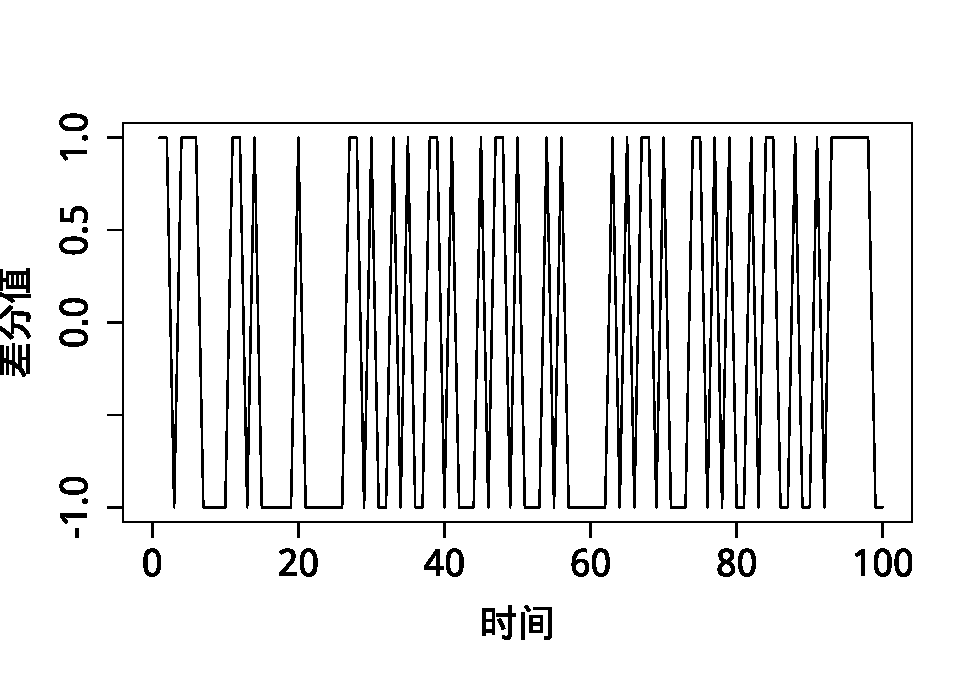
\includegraphics{time_series_files/figure-latex/unnamed-chunk-1-1.pdf}

\begin{Shaded}
\begin{Highlighting}[]
\KeywordTok{par}\NormalTok{(}\DataTypeTok{mfrow=}\KeywordTok{c}\NormalTok{(}\DecValTok{2}\NormalTok{,}\DecValTok{1}\NormalTok{),}\DataTypeTok{cex.axis=}\FloatTok{1.5}\NormalTok{,}\DataTypeTok{cex.lab=}\FloatTok{1.5}\NormalTok{)}
\KeywordTok{acf}\NormalTok{(x,}\DataTypeTok{main=}\StringTok{"随机游走模型"}\NormalTok{)}
\KeywordTok{acf}\NormalTok{(}\KeywordTok{diff}\NormalTok{(x),}\DataTypeTok{main=}\StringTok{"一阶差分序列"}\NormalTok{)}
\end{Highlighting}
\end{Shaded}

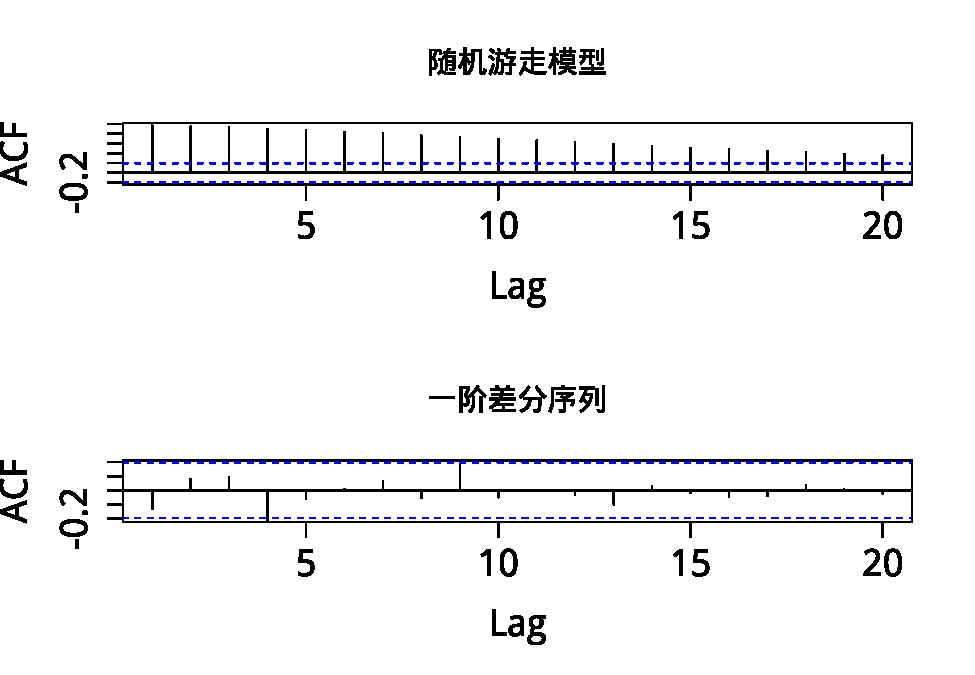
\includegraphics{time_series_files/figure-latex/unnamed-chunk-1-2.pdf}

\begin{Shaded}
\begin{Highlighting}[]
\KeywordTok{par}\NormalTok{(}\DataTypeTok{mfrow=}\KeywordTok{c}\NormalTok{(}\DecValTok{1}\NormalTok{,}\DecValTok{1}\NormalTok{))}

\KeywordTok{Box.test}\NormalTok{(}\KeywordTok{diff}\NormalTok{(x),}\DataTypeTok{lag=}\DecValTok{5}\NormalTok{,}\DataTypeTok{type=}\KeywordTok{c}\NormalTok{(}\StringTok{"Box-Pierce"}\NormalTok{))}
\end{Highlighting}
\end{Shaded}

\begin{verbatim}
->  
->      Box-Pierce test
->  
->  data:  diff(x)
->  X-squared = 7.8814, df = 5, p-value = 0.1629
\end{verbatim}

\begin{Shaded}
\begin{Highlighting}[]
\KeywordTok{Box.test}\NormalTok{(}\KeywordTok{diff}\NormalTok{(x),}\DataTypeTok{lag=}\DecValTok{5}\NormalTok{,}\DataTypeTok{type=}\KeywordTok{c}\NormalTok{(}\StringTok{"Ljung-Box"}\NormalTok{))}
\end{Highlighting}
\end{Shaded}

\begin{verbatim}
->  
->      Box-Ljung test
->  
->  data:  diff(x)
->  X-squared = 8.2976, df = 5, p-value = 0.1406
\end{verbatim}

\begin{Shaded}
\begin{Highlighting}[]
\NormalTok{index <-}\StringTok{ }\KeywordTok{ts}\NormalTok{(}\KeywordTok{read.csv}\NormalTok{(}\StringTok{"shindex.csv"}\NormalTok{,}\DataTypeTok{header =} \OtherTok{TRUE}\NormalTok{)[,}\DecValTok{2}\NormalTok{],}\DataTypeTok{start =} \KeywordTok{c}\NormalTok{(}\DecValTok{1995}\NormalTok{,}\DecValTok{1}\NormalTok{),}\DataTypeTok{frequency =} \DecValTok{12}\NormalTok{)}
\end{Highlighting}
\end{Shaded}

\end{document}
